%!TEX root = ../Bachelorarbeit.tex
\chapter{Umsetzung des Backends}

Die Umsetzung der gewählten Architektur und Konzepte in Project-Zoom ist Thema dieses Kapitels. Zuerst wird auf die Technologieauswahl eingegangen und die Implementierung des Data-centric Designs kurz erläutert. Anschließend wird die Realisierung der Anbindung der externen Komponenten an das Eventsystem am Beispiel verdeutlicht. Den Abschluss bildet Auswertung und erneute Betrachtung der Anforderungen. 

\section{Technologieauswahl}

\subsection{Scala im Web: Play Framework}
Die Auswahl der Programmiersprache wurde vor allem von dem Gedanken geprägt, eine Sprache zu finden, die einerseits auf benötigte Bibliotheken zugreifen kann und andererseits eine kurze Einarbeitungszeit benötigt. Für die Arbeit mit Thumbnails hat sich die Bibliothek Apache Tika als besonders wertvoll erwiesen. Nähere Informationen zu dieser Bibliothek finden sich in \cite{bp-dome}. Da diese Bibliothek in Java geschrieben wurde, musste die Wahl auf eine Sprache fallen, welche in der Lage ist, Java-Bibliotheken anzusprechen. 

Um die verschiedenen Sprachen und ihr jeweiliges Webframework zu evaluieren, wurde sich mit den in Tabelle \ref{tab:FrameWorkVergleich} aufgelisteten Kombinationen näher beschäftigt. Dazu wurde von den Backend-Entwicklern jeweils eine kurze Hello-World-Anwendung aufgesetzt. Dadurch konnte festgestellt werden, ob der Arbeitsablauf, der Aufwand und der zu erzeugende Quellcode angemessen sind. Neben dieser praktischen Kurzevaluierung wurden einige Fakten zusammengetragen, um die Entscheidung zu erleichtern. Die Kriterien Asynchronität und Zustandslosigkeit sind dabei vor allem im Kontext eines asynchronen Eventsystems von Interesse. Bezüglich der Indikatoren \tete{Adoption Ready}\footnote{Umfrage von InfoQ mit 1894 Teilnehmern auf \url{http://www.infoq.com/research/jvm-web-frameworks}. Erfragt wurde eine Einschätzung der Reife des Frameworks. Der Stand bei Abruf findet sich auf dem Bild \ref{fig:infoq-survey} im Anhang} und \tete{Importance}\footnote{Entnommen aus der bereits erwähnten InfoQ Umfrage. Erfragt wurde eine Einschätzung der Relevanz des Frameworks.} befinden sich alle Frameworks auf einem ähnlichen Niveau. 

In die nähere Auswahl kamen Java, Groovy und Scala\footnote{Mehr Informationen zu Scala und den Aspekten der Programmiersprache finden sich in \cite{scala-by-example}. Dieses Buch eignet sich sehr gut als Einstieg in die Programmiersprache.} mit den jeweiligen MVC Webframeworks Spring MVC\footnote{\url{http://www.springsource.org/features/modern-web}}, Grails\footnote{\url{http://grails.org}} und Play\footnote{\url{http://playframework.com}}. Im Gegensatz zu Spring und Grails ist Play ein zustandsloses, schlankes Framework, was eine ideale Voraussetzung für ein REST Backend darstellt. Zusätzlich spielten die persönlichen Präferenzen der Entwickler eine Rolle, die bereits Erfahrung in der Kombination Scala und Play hatten.

Scala ist eine Programmiersprache, deren Syntax an Java orientiert ist. Programme welche in Scala geschrieben sind, können bidirektional mit Java-Code interagieren und so auf den vollen Funktionsumfang der Java-Bibliotheken zurückgreifen. Dabei werden in der Sprache Konzepte der funktionalen mit gewohnten Elementen der objektorientierten Programmierung verknüpft.

\begin{tabularx}{\textwidth}{|p{0.2882\textwidth}|p{0.2\textwidth}|p{0.2\textwidth}|p{0.2\textwidth}|}
  \hline
  ~                                      & Java + Spring    & Groovy + Grails              & Scala + Play        \\\hline
  Authentifizierung                      & Ja mit Spring-WS & Ja mit Authentication Plugin & Ja mit SecureSocial \\\hline
  Json Unterstützung                     & Ja mit Jersey    & Ja                           & Ja                  \\\hline
  Vorhandene Erfahrung im Entwicklerteam & Gering           & Gut                          & Sehr Gut            \\\hline
  Dokumentation                          & Gut              & Gut                          & Gut                 \\\hline
  Asynchron                              & Nein             & Nein                         & Ja                  \\\hline
  Zustandslos                            & Nein             & Nein                         & Ja                  \\\hline
  \tete{Adoption Ready}                  & 85\%             & 77\%                         & 71\%                \\\hline
  \tete{Importance}                      & 82\%             & 76\%                         & 78\%                \\\hline
\end{tabularx}
\captionof{table}{Vergleich von verschiedenen Webframeworks miteinander\label{tab:FrameWorkVergleich}}

\subsection{MongoDB als Datenbanksystem}
Während der Prototypen-Phasen, in der sich die Idee der Umsetzung verfeinerte, wurde das bereits beschriebene Datenmodell aufgestellt. Ein wichtiger Aspekt, der für die Wahl der Datenbank entscheidend ist, sind die verschiedenen anbindbaren, externen Systeme. Das beschriebene Datenmodell verwendet flexible Datenstrukturen zur Speicherung von zusätzlichen Informationen zu Artefakten. Dies muss also auch durch die Datenbank unterstützt werden. Weiterhin müssen die Graphstrukturen in der Datenbank abgelegt werden. Dafür eignen sich besonders Datenspeicher, welche strukturierte Daten zulassen. Aus diesen Gründen fiel die Entscheidung auf eine NoSQL-Datenbank, welche die benötigte Flexibilität ohne großen Aufwand ermöglicht (vgl. \cite{mysgl-to-nosql}).

Neben der Open-Source Datenbank MongoDB\footnote{\url{http://mongodb.org}} stand Apache CouchDB\footnote{\url{http://couchdb.apache.org}} als Alternative zur Verfügung. Die Wahl von MongoDB als persistenten Speicher für Project-Zoom fiel vorrangig aufgrund des sehr guten Datenbank-Treibers ReactiveMongo\footnote{\url{http://reactivemongo.org}} für Scala. Dieser erlaubt komplett asynchrone Datenbankzugriffe und gliedert sich deshalb perfekt in das asynchrone Play Framework ein.

Als dokumentorientierter Datenspeicher passt MongoDB sehr gut zu einer REST-Architektur und dem Data-centric Design. Die Daten, welche in der Datenbank abgelegt werden, werden im Binary JSON (BSON)-Format gespeichert. Dieses BSON-Format ist eine binär encodierte Serialisierung von JSON-ähnlichen Dokumenten. BSON unterstützt die Repräsentation aller Datentypen, welche auch von JSON unterstützt werden, und erlaubt zusätzlich weitere Datentypen. So wurden die JSON-Datentypen unter anderem um die Unterstützung von Binärdaten und Datumsangaben erweitert (vgl. \cite{bson}). Somit ähnelt die Datenform, die auf Clientseite verarbeitet wird, dem Format der Datenspeicherung in der Datenbank. Diese Konstellation erlaubt die Implementierung einer schlanken Schicht des Datenmodells, wie sie im Abschnitt Data-centric Design \ref{sec:dcd} erklärt wurde.

\subsubsection{Zugriffsschutz für Datenbankobjekte}

Eine Anforderung der D-School bestand im Schutz der Daten (vgl. Anforderung \ref{itm:f1}). Diesen Schutz gilt es für die Objekte in der MongoDB umzusetzen. Dabei soll verhindert werden, dass Informationen aus Projekten für Personen, die kein Geheimhaltungsvertrag (NDA) für dieses Projekt unterschrieben haben, zugänglich sind. Studierende haben folglich nur Lesezugriff auf Projekte, an denen sie selbst teilgenommen haben oder die veröffentlicht\footnote{Aufgrund der fehlenden Einstellungsmöglichkeiten in der Filemaker Datenbank gibt es in der aktuellen Implementierung nicht die Möglichkeit ein Projekt als öffentlich zu kennzeichnen.} wurden. Schreibzugriff erhält ein Student nur als in der Filemaker-Datenbank vermerkter Teilnehmer des Projektes.

Bei der Betrachtung der Struktur von Zugriffsbeschränkungen fällt auf, dass diese abhängig von der zugriffssuchenden Person, der Art des Zugriffes und der Ressource sind. Basierend auf dieser Erkenntnis wurde ein sogenannter \tete{DBAccessContext} eingeführt. Für jeden Datenbankzugriff wird ein solcher Kontext benötigt. Mit Hilfe dessen können dann auf unterster Zugriffsebene, in den Funktionen \tete{insert}, \tete{update}, \tete{remove} und \tete{find}, die Berechtigungen überprüft werden.

Das Datenzugriffsobjekt für das jeweilige Datenmodell kann dann festlegen, wie mit Hilfe des DBAccessContext der Zugriff auf diese Methoden reguliert wird. Jedes dieser Datenzugriffsobjekte erbt von \tete{SecuredDAO}. In dieser Klasse findet die Ausführung der Datenbank Funktionen und die Zugriffsbeschränkung statt. Dadurch, dass die Zugriffsbeschränkungen für die jeweiligen Datenbankfunktionen einzeln festgelegt werden können, ist eine sehr feingranulare Differenzierung möglich.

Die Klasse \tete{SecuredDAO} überprüft die Berechtigungen wie folgt:
\begin{description}
\item[insert:] Beim Hinzufügen wird direkt kontrolliert ob der User die Berechtigung hat, neue Elemente in das jeweilige Datenmodell einzufügen. Fehlt diese, wird die Aktion mit einem Fehler abgebrochen
\item[update:] Eine Update-Aktion benötigt immer eine Suchanfrage und das eigentliche Update was auf die gefundenen Ergebnisse angewandt wird. Soll ein User nicht alle Objekte updaten können, so wird an die Suchanfrage die jeweilige Einschränkung angehangen. Damit wird verhindert, dass Objekte gefunden werden, auf die der User keinen Zugriff hat. Objekte die nicht gefunden werden, können demnach auch nicht verändert werden.
\item[find, remove:] Für das Abfragen und Löschen ist eine Suchanfrage notwendig. Diese wird genauso verändert wie dies für die \tete{update}-Funktion beschrieben ist. Der Ergebnisraum wird somit schon während der Abfrage auf die dem User zugänglichen Objekte beschränkt.
\end{description}

\subsection{Verwendete Bibliotheken}
Die umfangreichsten Bibliotheken, welche im Project-Zoom Backend Core verwendet werden, sind Akka\footnote{\url{http://akka.io}}, Play und SecureSocial\footnote{\url{http://securesocial.ws}}. Nicht hier aufgeführt ist ReactiveMongo als Datenbanktreiber. Diese Bibliothek wurde bereits im Abschnitt \ref{sec:reactive} näher erläutert. 

\paragraph{Akka}\label{sec:actor} stellt die Grundlage für das Play Framework dar. Die Bibliothek ermöglicht die Nutzung verschiedener Konzepte des asynchronen Programmierens. Das Ziel ist, das Schreiben von parallelen, fehlertoleranten und skalierbaren Anwendungen zu vereinfachen \cite{what-is-akka}. 

Die sogenannten \tete{Actors}\footnote{Die Idee von Aktoren wurde erstmals in \cite{actors} beschrieben} der Bibliothek sind für dieses Projekt am relevantesten. Sie stellen eine Implementierung des Aktorenmodells dar. Aktoren sind abgeschlossene Einheiten, welche nur über Nachrichten kommunizieren. Dabei erfolgt die Abarbeitung der Nachrichten eines Aktors sequenziell, die Kommunikation mit anderen Aktoren hingegen asynchron. Dadurch können mehrere Nachrichten in unterschiedlichen Aktoren gleichzeitig abgearbeitet werden. Verschiedene Aktoren teilen sich nur über Nachrichten ausgetauschte Variablen. Damit das System also threadsicher arbeitet, müssen diese Nachrichten threadsicher sein. In Scala ist es deshalb üblich, für Nachrichten \tete{Case Classes}\footnote{\url{ http://www.scala-lang.org/node/107 }} zu verwenden. Diese sind von vornherein unveränderbar und somit threadsicher.

Neben Actors finden auch \tete{Agents} in Project-Zoom Verwendung. Ein Agent bildet eine Kapselung um einen Zustand. Dieser Zustand kann unverzüglich synchron gelesen und asynchron überschrieben werden. Bei einem Update wird dem Agent eine Funktion übergeben, welche den neuen Zustand des Agents berechnet. Einen Agent kann man zum Beispiel verwenden um Zustand zwischen verschiedenen Actors zu teilen.

\paragraph{Play Framework 2.0} ist die Weiterentwicklung  und Portierung eines früheren Java Web Frameworks nach Scala. Es ist zwar in Scala programmiert, kann aber sowohl mit Java als auch Scala als Backend Sprache verwendet werden. Play liegt eine MVC Architektur zugrunde. Hierbei werden in jedem Controller sogenannte \tete{Actions} definiert und im View verschiedene \tete{Templates} angelegt. Der Ablauf einer Anfrage an den Webserver verläuft wie folgt:

\begin{enumerate}
  \item Der standardmäßige HTTP-Router leitet die Anfrage an eine Action weiter. Diese Weiterleitung basiert auf den Routen, die in der Datei conf/routes definiert sind.
\begin{lstlisting}
GET   /projects/:id   ProjectController.read(id: String)
\end{lstlisting}
Eine Route besteht dabei immer aus einer der HTTP-Methoden GET, POST, HEAD, PUT oder DELETE (vgl. \cite{play-scala-routing}), einem URI-Pattern und einer Action, die den Request beantwortet.
\item Die Action im Controller ist für die Beantwortung zuständig. Dazu können Informationen im Model abgefragt werden. Die Templates können benutzt werden, um ein dynamisches Ergebnis für den Client zu erzeugen.
\end{enumerate}

\paragraph{SecureSocial} umfasst den User-Login. Dieses Paket ist ein Authentifizierungsmodul mit Support für OAuth\footnote{OAuth, \url{https://tools.ietf.org/html/rfc5849}}, OAuth2 \footnote{OAuth2 \url{https://tools.ietf.org/html/rfc6749}}, OpenID\footnote{OpenID, \url{http://openid.net/specs/openid-authentication-2_0.html}} und Username/Passwort-Authentifizierung. 

\subsection{Modularisierung}
Play erlaubt die Modularisierung des Codes in sogenannte Subprojekte. Ein solches Subprojekt ist dabei eine abgeschlossene Einheit, welche allein kompiliert, getestet und ausgeführt werden kann. Dabei können neben Play-Projekten auch Java- oder Scala-Projekte als Subprojekte verwendet werden. Die einzelnen Projekte und deren Abhängigkeiten werden in der \tete{Build.scala}-Datei angegeben.
Project-Zoom besteht aus drei verschiedenen Subprojekten:

\paragraph{common} enthält den Quelltext der sowohl von den Projekten \tete{main} als auch \tete{admin} benötigt wird. In diesem Projekt sind die Datenmodelle definiert. Weiterhin befinden sich in diesem Modul das Eventsystem, die Erweiterungen zum Datenaggregieren und zum Thumbnailgenerieren, sowie die Authentifizierung.

\paragraph{main} schließt alle Controller ein, die für den normalen Nutzer ansprechbar sind. Es wurden verschiedenen Actions definiert und für die jeweiligen Sichten Templates angelegt. Der Frontend-Code, welcher näher in den Arbeiten \cite{bp-norman}, \cite{bp-tomh} und \cite{bp-anita} beschrieben ist, wird ebenfalls in diesem Projekt verwaltet.

\paragraph{admin} definiert jede Interaktion, die nur 
für privilegierte Nutzer sichtbar sein soll. Dies sorgt für eine klare Trennung zwischen User- und Admin-Anfragen und gewährleistet mehr Sicherheit (vgl. Anforderung \ref{itm:f1}). Ein weiterer Vorteil ist, dass durch das Abschalten dieses Subprojektes jedwede Admin-Aktion unterbunden werden kann.

\begin{figure}[h]  
  \centering     
  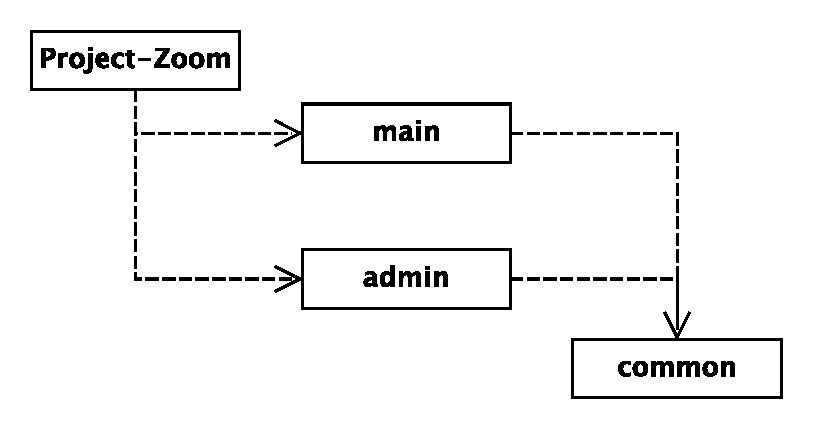
\includegraphics[width=0.8\textwidth]{img/projekte.pdf}  
   \caption{Projekte und deren Abhängigkeiten}   
  \label{fig:projects} 
\end{figure}

\FloatBarrier
In der Grafik \ref{fig:projects} sind die Abhängigkeiten der Pakte voneinander dargestellt. Das Anlegen eines Hauptprojektes, in diesem Fall Project-Zoom, erleichtert die Arbeit mit dem Gesamtprojekt. Durch die Abhängigkeit zu \tete{main} und \tete{admin} muss nur noch das Hauptprojekt kompiliert werden, denn die Abhängigkeiten werden bei Source-Code Änderungen automatisch mit kompiliert.

\section{Data-centric Design in Project-Zoom}
\label{sec:umsetzung_dcd}
Die REST-Schnittstelle von Project-Zoom entspricht der einer klassischen CRUD-Anwendung. Aufgrund der geringen Business-Logik liegt es nahe, das beschriebene Data-centric Design zu verwenden. Um die Wartung des Systems zu erleichtern, werden Datenzugriffsobjekte für jedes Datenmodell verwendet.

\lstinputlisting[caption=Macro Verwendung zur Generierung einer JSON Konvertierung, label=lst:json-format, language=scala]{code/json_reads.scala}

Für einige Teile der Anwendung ist es notwendig die JSON-Strukturen der Datenbank in Scala-Objekte umzuwandeln. Dies ist zum Beispiel für User Objekte der Fall, welche von der Authentifizierungsbibliothek SecureSocial verwendet werden. Play erlaubt die Generierung der Transformationsfunktionen mit Hilfe von Macros\footnote{JSON Macro incepetion \url{http://www.playframework.com/documentation/2.1.1/ScalaJsonInception}}. Das bedeutet, dass die Anwendung die Datenklassen des Modells definiert und die Funktionen zur Konvertierung von und nach JSON während der Kompilierung vom Framework übernommen werden. Ein Beispiel für solch eine Transformation ist in \ref{lst:json-format} mit der Variablen \tete{userFormat} gegeben. Diese ist in der Lage, zwischen den beispielhaften Repräsentationen 
\begin{lstlisting} 
{ 
  "firstName" : "Max", 
  "lastName"  : "Mustermann" 
}
\end{lstlisting} und 
\begin{lstlisting} 
User("Max", "Mustermann")
\end{lstlisting} 
zu konvertieren. Diese Bedarfskonvertierung ist durch die Verwendung von unveränderbaren Case-Klassen typsicher und entspricht den Konzepten der funktionalen Programmierung \cite{functional-thinking}.

Die CRUD-Operationen \tete{list} und \tete{read} wurden implementiert, ohne Datenbankobjekte zu konvertieren. Die Daten werden aus der Datenbank gelesen, transformiert und anschließend an den anfragenden Clienten zurückgegeben. Bei der Transformation werden z.B. Passwort-Hashes und Login-Informationen, die sich im User-Objekt befinden, entfernt. Die Funktionen \tete{create}, \tete{update} und \tete{delete} sind nicht für alle Datenbankobjekte implementiert. Dies liegt an der Anforderung, dass die Datenhaltung in der von der D-School bereits verwendeten Datenbank geschehen soll. Project-Zoom soll diese Daten nur aggregieren.


\section{Anbindung externer Komponenten}

Die Implementierung des Eventsystems zur Anbindung externer Komponenten in Project-Zoom basiert auf dem Akka-Framework. Die in Absatz \ref{sec:actor} beschriebenen Aktoren eignen sich sehr gut zur Modellierung eines Subscribers. Ein Aktor ist eine abgeschlossene funktionelle Einheit, deren Kommunikation nur über unveränderbare Nachrichten erfolgt. Erhält ein Aktor eine Nachricht, so wird diese in der Mailbox gesammelt. Die Nachrichten in der Mailbox werden dann mit Hilfe der \qc{receive}-Funktion, welche jeder Aktor definieren muss, abgearbeitet. 

In der Umsetzung erfolgt das Abonnieren einer Nachricht durch das Senden einer partiellen Funktion\footnote{Eine partielle Funktion $f: A \rightarrow B$ ist im Gegensatz zu einer totalen Funktion nicht auf jedem Wert aus $A$ definiert. Für die Anwendung in Scala siehe \cite{partial-function})} an den Dispatcher. Diese Funktion bildet den Typ \tete{Event} auf Unit ab und ist auf allen Events definiert, welche der Subscriber empfangen will. Der Dispatcher benutzt anschließend alle partiellen Funktionen, um eine eingehende Nachricht zu verteilen. Standardmäßig hat ein Subscriber alle Nachrichten abonniert, für die seine \qc{receive}-Funktion definiert ist.

\subsection{Anbindung der Konnektoren und des Thumbnailgenerators}

Externe Komponenten kommunizieren untereinander und mit dem Core über dieses gerade beschriebene Eventsystem. Ein Beispiel solch einer Kommunikation ist in der Abbildung \ref{fig:eventsystem-bsp} zu sehen. Der Ablauf zeigt wie ein Konnektor ein neues Artefakt registriert, welches anschließend vom Core und vom Thumnailsystem verarbeitet wird. Eine Übersicht über alle vom Backend-Core empfangenen und gesendeten Events findet sich im Anhang \ref{event-overiview}.

\begin{figure}[h]  
  \centering     
  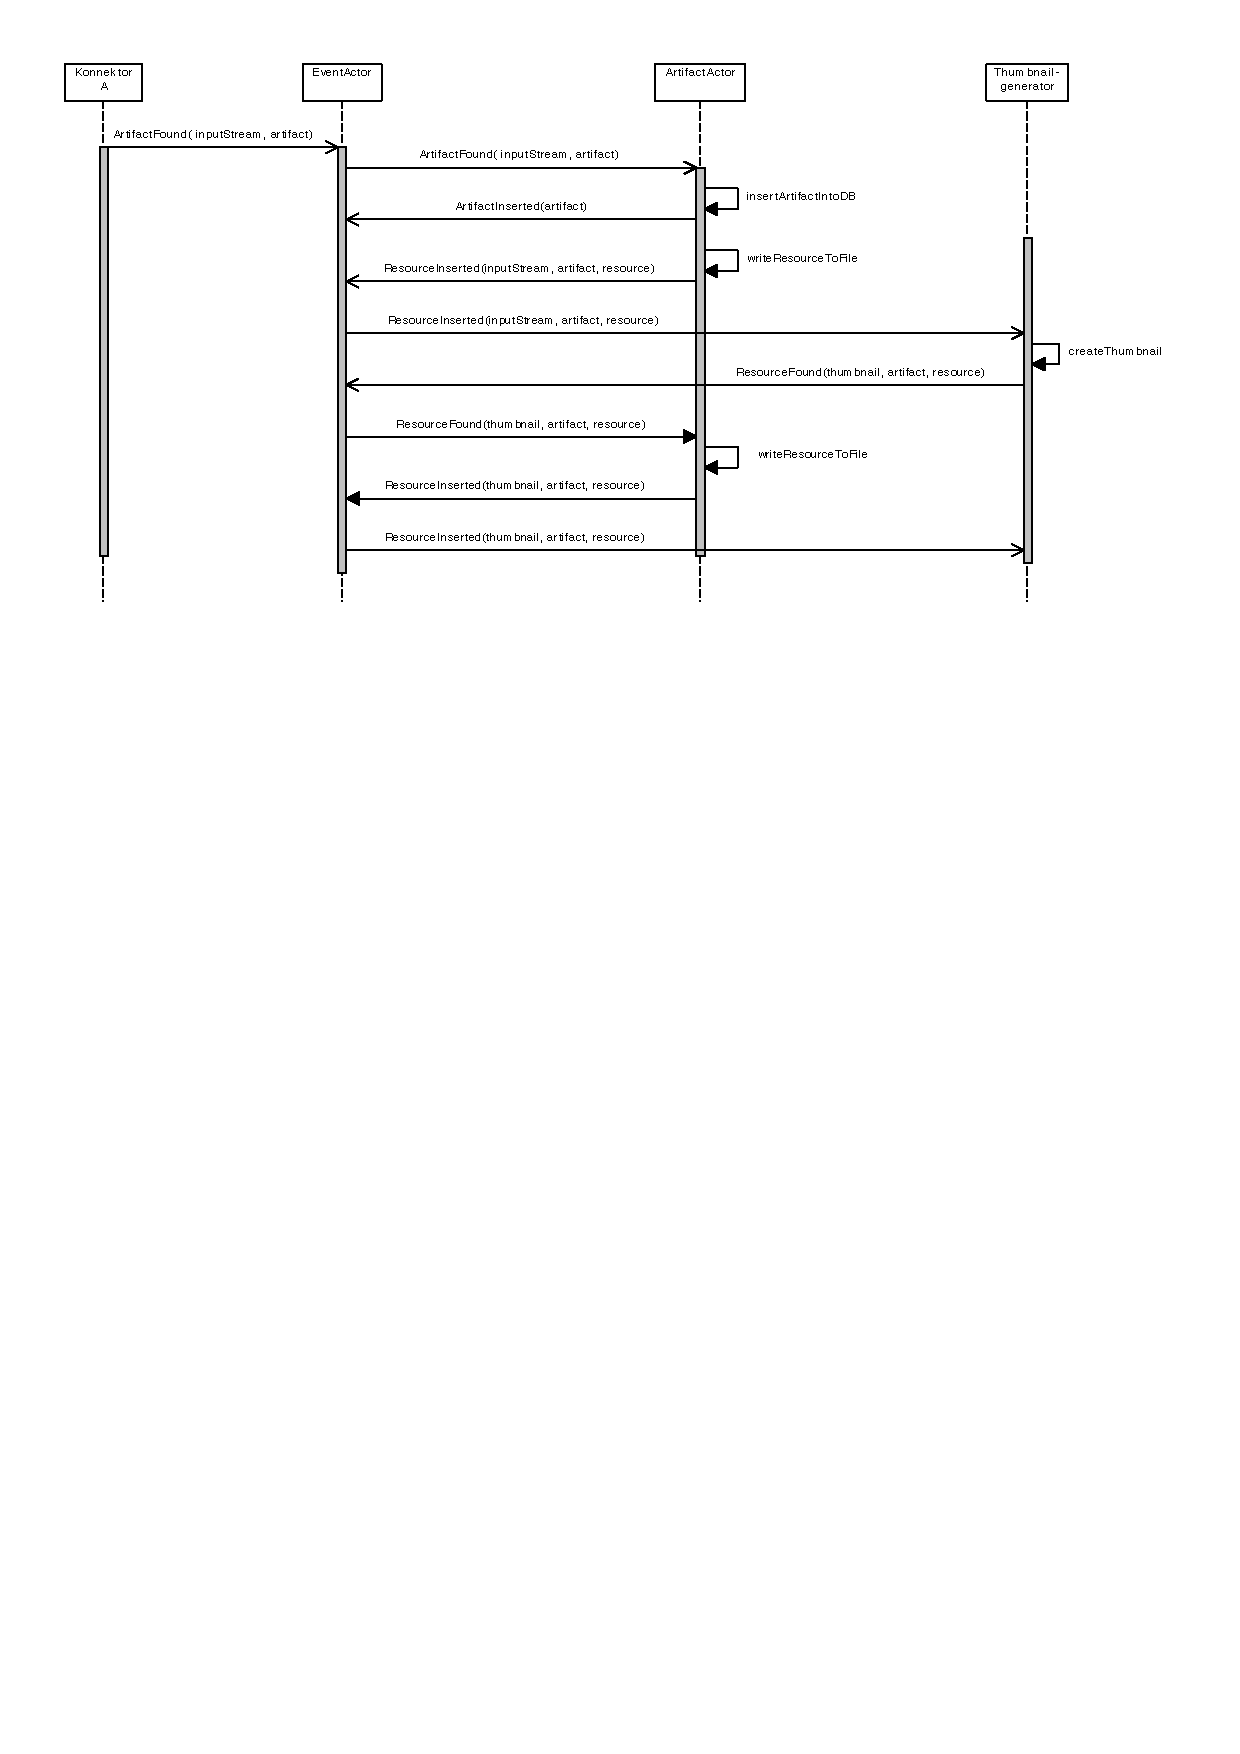
\includegraphics[width=1.0\textwidth]{img/eventsystem_bsp.pdf}  
   \caption{Beispielhafter Ablauf beim Fund eines neuen Artefaktes}   
  \label{fig:eventsystem-bsp} 
\end{figure}

\section{Evaluierung der Requirements}

Den Abschluss der Implementierungsbetrachtungen soll ein Rückblick auf die im Abschnitt \ref{sec:requirements} aufgestellten Anforderungen an das System bilden.

Es wurde ein System entwickelt, welches zur Trennung von Administration und Nutzung in Module geteilt ist. Die Webanwendung ist durch das Authentifizierungsmodul SecureSocial und die Implementierten Autorisierungsmechanismen in den Datenbankzugriffsobjekten geschützt (vgl. Anforderung \ref{itm:f1}). Die Anwendung ist aus dem Internet erreichbar und somit auch von außerhalb der D-School (vgl. Anforderung \ref{itm:f6})

Bei der Umsetzung der Konnektoren (vgl. Anforderung \ref{itm:f2}) sei auf die Arbeit von Thomas Werkmeister \cite{bp-tewe}, in welcher die umgesetzten Konnektoren erläutert sind. Die Datenquellen die in \cite{bp-tewe} beschrieben sind, werden durch die Aggregation nicht verändert (vgl. Anforderung \ref{itm:f5}). Anforderung \ref{itm:f3} fordert, dass keine Daten gelöscht werden. Dies wurde umgangen, indem beim Löschen von Elementen aus einer aggregierten Datenquelle die entsprechenden Artefakte als gelöscht markiert werden.

Die Anforderung \ref{itm:f4} fordert die einfache Anbindbarkeit von neuen Datenquellen. Durch das Eventsystem, welches durch das Backend zur Verfügung gestellt wird, steht ein System zur Verfügung, was viel Spielraum für das Anbinden neuer Konnektoren bietet.

Um die maximale Last des Systems zu prüfen, wurde mit Hilfe von \tete{Apache HTTP Bench}\footnote{\tete{ab} - Apache HTTP Server Benchmarking Tool \url{http://httpd.apache.org/docs/2.2/programs/ab.html}} ein Lasttest ausgeführt. Bei diesem Test wurde eine maximale Last mit im Durchschnitt 461 Anfragen pro Sekunde ermittelt (vgl. Anforderung \ref{itm:nf1}). Nähere Informationen und Ergebnisse finden sich im Anhang \ref{sec:performance-test}.

Die Aktualisierung der angebundenen Datenquellen erfolgt einmal pro Minute (vgl. \cite{bp-tewe}). Damit ist auch die Anforderung \ref{itm:nf2} erfüllt.